\begin{figure}[t!]
	\centering
	\begin{subfigure}[t]{0.4\textwidth}
		\centering
		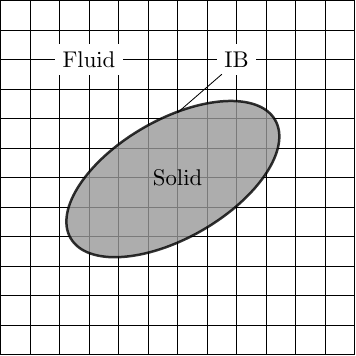
\includegraphics[width=1\linewidth]{images/IBM.png}
		\caption{Non-conforming mesh method in IBM}
	\end{subfigure}%
	~ 
	\begin{subfigure}[t]{0.5\textwidth}
		\centering
		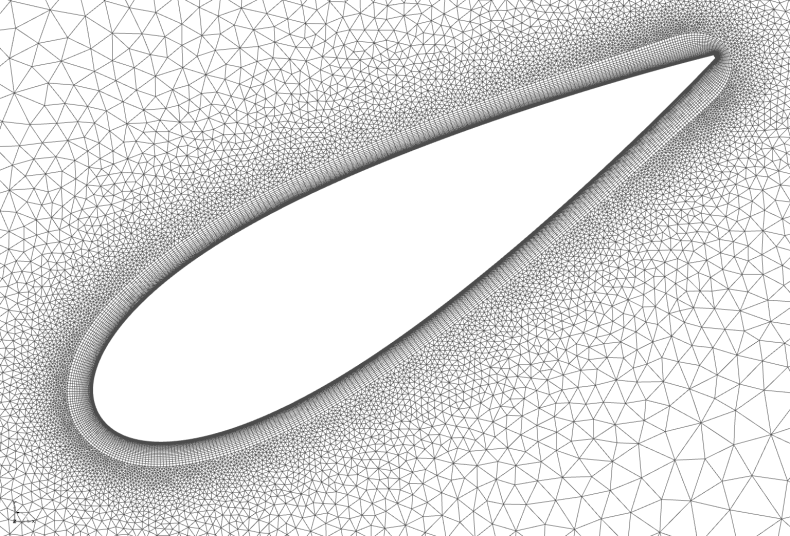
\includegraphics[width=1\linewidth,height=0.8\linewidth]{images/ConformingMesh.png}
		\caption{Conforming mesh method}
	\end{subfigure}
\caption{Illustration of the computational domains for non-conforming and conforming mesh methods.}
\label{fig:FSI_lit}
\end{figure}